\documentclass[ a4paper, 
                amsfonts, 
                amssymb, 
                amsmath, 
                reprint, 
                showkeys, 
                nofootinbib,
                superscriptaddress, 
                %twoside,
                onecolumn, 
                notitlepage,
                aps,
                pra,
                longbibliography]{revtex4-1}
                
\usepackage[margin=1in]{geometry}
\usepackage{amsmath,amssymb,amsthm}
\usepackage{braket}
\usepackage{xcolor}
\usepackage{amsthm}
\usepackage{graphicx}

\usepackage{algorithm}
\usepackage{algorithmic}

\usepackage[colorlinks]{hyperref}
\usepackage[capitalise]{cleveref}

%\definecolor{blue}{rgb}{0,0,1}
\newcommand{\yu}[1]{\textcolor{blue}{#1}}
\newcommand{\tom}[1]{\textcolor{purple}{#1}}
\newtheorem{question}{Question}
\newtheorem{oquestion}{Open question}
\newtheorem{theorem}{Theorem}
\newenvironment{equation-aligned}{\begin{equation}\begin{aligned}}{\end{aligned}\end{equation}}



\theoremstyle{definition}
\newtheorem{definition}{Definition}[section]  
% \newtheorem{definition}{Definition}      
\newcommand{\bC}{{\mathbb{C}}}
\newcommand{\bR}{{\mathbb{R}}}
\newcommand{\bN}{{\mathbb{N}}}
\DeclareMathOperator{\Tr}{Tr}




\begin{document}

\title{Autonomous state reachability}


% feel free to permute the order of authors

\author{Tomasz Andrzejewski}
\email{tomasz.andrzejewski@tuwien.ac.at}
\affiliation{Atominstitut, Technische Universit{\"a}t Wien, Stadionallee 2, 1020 Vienna, Austria}

\author{Yuri Minoguchi}
\email{}
\affiliation{Atominstitut, Technische Universit{\"a}t Wien, Stadionallee 2, 1020 Vienna, Austria}


% I don't wanna put myself on there :p that's for you guys to decide
\author{Phila Rembold}
\email{}
\affiliation{Atominstitut, Technische Universit{\"a}t Wien, Stadionallee 2, 1020 Vienna, Austria}

\author{Konrad Szymanski}
\email{konrad.szymanski@quantumstat.es}
\affiliation{Research Center for Quantum Information, Bratislava}



\begin{abstract}

\end{abstract}

\date{\today}

\maketitle

\maketitle

\section{Basic problem statement}
The original question which spurred this research is the following: 
\begin{question}
Can every quantum state be approximated arbitrarily well by autonomous evolution of product states under 2-body Hamiltonians?
\end{question}
There are various ways to make this concrete. One could talk about different systems (e.g, $N$ qubits, or indistinguishable particles), different allowed Hamiltonian families (all allowed 2-body interactions, or restricted subset, or possibly abstract subspace of Hermitian operators without much physical interpretation).

Mathematically, I decided to formulate it as below. For simplicity, the initial state is considered fixed, and only the Hamiltonians are allowed to change.

\begin{question}
Let us fix a Hamiltonian family $H=\sum_{k=1}^n \lambda_k H_k$, with free parameters $\lambda_1, \ldots, \lambda_n$. The target state is $\ket\psi$, and an initial state is denoted by $\ket\phi$. Given arbitrary $\varepsilon > 0$, does there exist a selection of parameters $\lambda_1, \ldots, \lambda_n \in \mathbb{R}^n$ such that

\begin{equation}
|\ket{\psi} - \exp(-i\sum_{k=1}^n \lambda_k H_k)\ket{\phi}| < \varepsilon?
\end{equation}
\label{q:act}
\end{question}
In the $N$ qubit setup, one can consider simple heurestic reasoning like \textbf{parameter counting}. Every $2$-body Hamiltonian can be written as 
\begin{equation}
H = \sum_{1\le i<j\le N} \sum_{\alpha,\beta=1,2,3} \lambda_{i,j;\alpha,\beta} \sigma_{\alpha}^{(i)} \otimes \sigma_{\beta}^{(j)} +  \sum_{1\le i \le N} \sum_{\alpha=1,2,3} \lambda_{i;\alpha} \sigma_{\alpha}^{(i)} ,\label{eq:nqbham}
\end{equation}
and the number of parameters is quadratic -- it is dominated by the qubit pairs in the first part of the equation. On the other hand, the number of parameters needed to specify a state of $N$ qubits grows exponentially. As a result, for $N \geq 7$ qubits, it seems that given fixed initial state, there is no enough parameters to reach arbitary states. 

The above is just a heurestic --- the question is \emph{how to prove unreachability}. In the following section, I present one method I devised in the last year.

\section{Moment-based detection {criterion for} unreachability}
If the conditions of \cref{q:act} apply, necessarily there must exist a choice of the parameters $\lambda_1, \ldots, \lambda_n$ for the Hamiltonian $H:=\sum_{k=1}^n \lambda_k H_k$ such that the moments of the initial and final states coincide:
\begin{equation}
\braket{H^l}_\psi = \braket{H^l}_\phi \quad \forall l \in \bN.
\end{equation}
Considering the Hamiltonian $H$ is a linear expression in the parameters $\lambda_1, \ldots, \lambda_n$, this leads to a polynomial feasibility condition:

\begin{theorem}
 Fix the initial $\ket\phi$ and target state $\ket{\psi}$. If the pair of states is reachable in the sense of  \cref{q:act}, there must exist a choice of parameters $\lambda_1, \ldots, \lambda_n \in \mathbb{R}^n$ such that
\begin{equation}
\sum_{(i_1, \ldots, i_n) \in S_l} \lambda_1^{i_1} \cdot \ldots\cdot \lambda_n^{i_n} (\langle H_1^{i_1} \cdot \ldots\cdot H_n^{i_n}\rangle_{\psi}-\langle H_1^{i_1} \cdot \ldots\cdot H_n^{i_n}\rangle_{\phi})=0, ~~~\forall l\in\mathbb{N}\label{eq:restrcond}
\end{equation}
where the summation goes over indices summing up to $l$:
\begin{equation}
S_l = \{(i_1,\ldots,i_n)\in\mathbb{N}^n : i_1+\ldots+i_n = l\}.
\end{equation}\label{thm:allmom}
\end{theorem}
Even with the states $\ket\psi$ and $\ket\phi$ fixed and with a restricted, but nontrivial set of Hamiltonians $H_1, \ldots, H_n$, this is computationally really complex condition. However, it can be substantially simplified: the \cref{eq:restrcond} has to hold for all $l$, and in particular $l=1,2$. Consideration of only the first two moments greatly simplifies calculations and is often enough to detect unreachability, as shown below.
\begin{theorem}
\label{main}
 Fix the initial $\ket\phi$ and target state $\ket{\psi}$ and write out the polynomials appearing in \cref{eq:restrcond} for $l=1,2$ explicitly:
\begin{equation-aligned}
L &:= \sum_{k=1}^n \lambda_k (\braket{H_k}_\psi -\braket{H_k}_\phi),\\
Q&:= \sum_{k,m=1}^n \lambda_k\lambda_m (\braket{\frac12\{H_k,H_m\}}_\psi -\braket{\frac12\{H_k,H_m\}}_\phi),
\end{equation-aligned}

where $\{\cdot, \cdot\}$ denotes the anticommutator. If there exists $x\in\mathbb{R}$ such that $Q+ x L^2$ is positive \textbf{definite} as a quadratic function of $\lambda_1, \ldots, \lambda_n$, the state $\ket\psi$ is unreachable from $\ket\phi$.
\label{thm:twomom}
\end{theorem}
The above is a consequence of the fact that if $Q+ x L^2$ is positive definite for some $x$, it is impossible for both $L=0$ ($\Leftrightarrow$ first moment match) and $Q=0$ ($\Leftrightarrow$ second moments match), unless $\lambda_1 = \ldots = \lambda_n = 0$, which is no dynamics at all.

\subsection{Example: $N$ bosons in 2 modes}
\newcommand{\hc}{\text{h.c.}}
Consider the case of $N$ bosons in 2 modes (denoted by annihilation operators $a$ and $b$), with the following Hamiltonians spanning the allowed interactions (they are single-body hopping terms, local energies, and two-body interactions, with redundancies removed):
\begin{equation-aligned}
 H_1&=a^\dagger b + b^\dagger a,&H_2 = i (a^\dagger b- b^\dagger a),&~H_3 = a^\dagger a-b^\dagger b,\\
H_4&= \{H_1, H_2\}, &H_5 = \{H_1,H_3\},  &~H_6= \{H_2, H_3\},\\
H_7&=H_1^2,&& H_8=H_2^2.
\end{equation-aligned}
For $N \geq 7$ bosons, I am able to prove that there exist states unreachable from 
\begin{equation}
\ket\phi = \ket{N,0} = (a^\dagger)^N\ket{\emptyset}.
\end{equation}
One of them is 
\begin{equation}
\ket{\psi} = \frac{1}{\sqrt{2}}(\ket{N,1} + \ket{1,N}).
\end{equation}
This is a direct application of \cref{thm:twomom}: in such case one can find $x$ such that $Q+xL^2$ is positive definite, implying the first two moment of the Hamiltonian $H=\sum_{k=1}^8 \lambda_k H_k$ can never match for the two states simultaneusly. This proves unreachability.




\subsection{Example: random states in 1D Ising model}
The system is composed of $N$ sites, with the Hamiltonian given as 
\begin{equation}
H =  \sum_{i=1}^N \lambda_i \sigma_z^{(i)} \sigma_z^{(i+1)} + \lambda_{N+1} \sum_{i=1}^N \sigma_x^{(i)},\label{eq:ising1}
\end{equation}
with cyclic boundary conditions ($N+1 = 1$). So, the interaction strength between adjacent sites is allowed to vary, but the transverse field is constant. I investigated the probability of unreachability detection using the two-moment criterion (\cref{thm:twomom}), with 
\begin{equation}
\ket\phi = \ket{0}^{\otimes N}\label{eq:isinginit}
\end{equation}
as the initial state, and final states $\ket\psi$ being drawn uniformly from the sphere of pure states. The results are as follows:\\
\begin{figure}[!h]
\centering
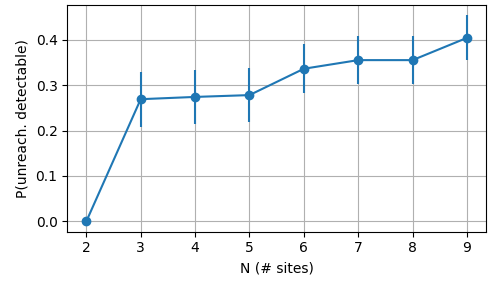
\includegraphics[width=.6\linewidth]{ising.png}
\caption{Probability (rough Monte Carlo estimate) of unreachability detection in the Ising model (\cref{eq:ising1}), starting from initial product state described by \cref{eq:isinginit}. The target states are sampled uniformly from unit sphere in $\mathbb{C}^{2^N}$. }
\end{figure}~\\
There are finitely many sampled random final states $\ket\psi$, so naturally there some numerical noise is present. The shot noise ($\approx ({\text{number of samples}})^{-\frac12}$) is indicated with errorbars. Still, it seems that even with simplified criterion around $\frac13$ of the states can be proved to be unreachable.



\subsection{Example: GOE Hamiltonians and random states in $d$-dimensional space}
\yu{Let us focus on a single $d$-dimensional Hilbert space with $H = \sum_{i=1}^{d^2} 
\lambda_i g_i$ where $g_i$ are the $d^2$ generators of the Lie group $U(d)$. 
One choice could be $g_i \in \{ \vert n \rangle \langle m \vert \}_{m,n=1}^{d}$.
Another choice which may be more favorable for an analytical treatment are randomly rotated generators $g_i$ could be $g_i \in \{ U_m \vert 0 \rangle \langle 0 \vert V_n\}_{m,n=1}^d$ where $U,V \in \mathrm{CUE}(d)$ which corresponds to the $d$-dimensional circular unitary ensemble. For $d \gg 1$ the generators will be approximately orthogonal. This approach may be further simplified by considering a family of $d$ random projections $g_i \in \{ U_i\vert 0 \rangle \langle 0\vert U_i^\dagger \}_{i=1}^d $.
}
One may further deform this choice by considering a family of \emph{random} Hamiltonians. Here we fix $d$, the total dimension, and $n$, the number of Hamiltonians. Then, $n$ Hamiltonians $H_1, \ldots, H_n$ are sampled from Gaussian Orthogonal Ensemble \footnote{Surprisingly, the results are almost identical if \emph{random projectors} $H_k=\ket{\alpha_k}\bra{\alpha_k}$ are sampled instead (or random matrices from Gaussian Unitary Ensemble, for that matter).}. That is, if $X$ is a square matrix of size $d$, with $X_{i,j}$ sampled i.i.d. from standard normal distribution $\mathcal{N}(0,1)$, 
\begin{equation}H_k = \frac{X+X^T}{\sqrt{2}},\end{equation}
and each $H_k$ is sampled independently. The target state $\ket\psi$ is sampled uniformly from unit sphere in $\mathbb{C}^d$. The initial state can be fixed, since everything else (the Hamiltonian and final state sampling) is sampled from unitary invariant measures, therefore always
\begin{equation}
\ket\phi = \begin{pmatrix} 1\\0\\\vdots\\0\end{pmatrix} \in\mathbb{C}^d.
\end{equation}
The question here is: what is the probability $P_{d,n}$ of a randomly sampled state $\ket\psi\in\mathbb{C}^d$ {to be reachable from $\ket\phi$ with Hamiltonian $H=\sum_{k=1}^n \lambda_k H_k$ composed of random matrices} $H_1, \ldots, H_n$? Here are the results of a Monte Carlo simulation.
\begin{figure}[!h]

\centering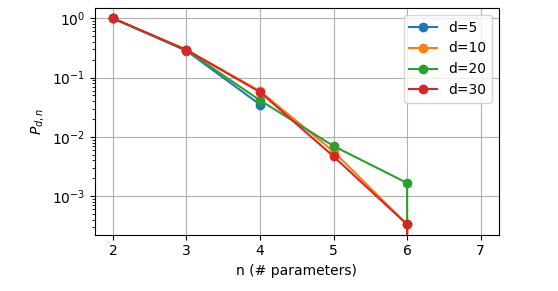
\includegraphics[width=.7\linewidth]{random_goe.png}
\caption{\label{fig:random_goe} Probability (\textbf{very} rough Monte Carlo estimate) of unreachability detection in the random matrix model. The shot noise is substantial, especially for low probabilities, but it is hard to show it on this plot (there are many overlapping points). Notable is that the decay is exponential and does not seem to strongly depend on $d$.}
\end{figure}
Interestingly, there is an exponential falloff of unreachability detection probability $P_{d,n}$ as a function $n$ (the number of Hamiltonian parameters), without much dependence on $d$ (the dimension), at least during the initial falloff. Naturally, once $n\ge d^2-1$, generically any Hamiltonian can be produced, and in turn, any unitary and any target state. However, it is nontrivial to numerically probe the onset of zero probability due to huge shot noise when sampling rare events.
\begin{oquestion}
Why does the unreachability probability decay exponentially with $n$?
\end{oquestion}
\yu{
\begin{oquestion}
How would this curve look when we allow full time dependent control?
\end{oquestion}
}
\yu{
\begin{oquestion}
Is it possible to map this to the statistical physics of a perceptron where the unreachability can be encoded population in ground state? With this one could attempt to obtain an analytical derivation of the exponential decay.
\end{oquestion}
}


    \subsection{Spectral-Overlap Criterion}

Given a Hamiltonian family $H(\boldsymbol{\lambda}) = \sum_{k=1}^K \lambda_k H_k$ with parameters $\boldsymbol{\lambda} \in [-1,1]^K$, we diagonalize 
\begin{equation}
U(\boldsymbol{\lambda})^\dagger H(\boldsymbol{\lambda}) U(\boldsymbol{\lambda}) = \mathrm{diag}(E_1, \ldots, E_d)
\end{equation}
to obtain the eigenbasis $\{|n(\boldsymbol{\lambda})\rangle\}_{n=1}^d$. The initial state $|\varphi\rangle$ and target state $|\psi\rangle$ can be expanded in this basis:
\begin{equation}
|\psi\rangle = \sum_{n=1}^d \psi_n(\boldsymbol{\lambda}) |n(\boldsymbol{\lambda})\rangle, \quad |\varphi\rangle = \sum_{n=1}^d \varphi_n(\boldsymbol{\lambda}) |n(\boldsymbol{\lambda})\rangle
\end{equation}
where $\psi_n(\boldsymbol{\lambda}) = \langle n(\boldsymbol{\lambda})|\psi\rangle$ and $\varphi_n(\boldsymbol{\lambda}) = \langle n(\boldsymbol{\lambda})|\varphi\rangle$ are complex amplitudes.

The  spectral overlap is defined as:
\begin{equation}
S(\boldsymbol{\lambda}) = \sum_{n=1}^d \left|\varphi_n(\boldsymbol{\lambda})^* \psi_n(\boldsymbol{\lambda})\right|
\label{eq:spectral_overlap_correct}
\end{equation}

The maximized spectral overlap
\begin{equation}
S^* = \max_{\boldsymbol{\lambda} \in [-1,1]^K} S(\boldsymbol{\lambda})
\end{equation}
quantifies the best alignment achievable between the amplitude distributions of initial and target states across all eigenbases attainable by the Hamiltonian family.

We say that a target state $|\psi\rangle$ is \textbf{reachable} from initial state $|\varphi\rangle$ if:
\begin{equation}
S^* \geq \tau
\end{equation}
where $\tau \in [0.90, 0.999]?$ is a fixed threshold (taken to be $\tau = 0.95$).

The unreachability probability for dimension $d$ with $K$ control Hamiltonians is estimated via Monte Carlo:
\begin{equation}
P_{\text{unreach}}^{\text{new}}(d, K; \tau) = \Pr\left[ \max_{\boldsymbol{\lambda} \in [-1,1]^K} S(\boldsymbol{\lambda}) < \tau \right]
\end{equation}
where the probability is over random Hamiltonian sets $\{H_k\}_{k=1}^K$ sampled from GOE or GUE, and random target states $|\psi\rangle$ sampled uniformly from the unit sphere in $\mathbb{C}^d$, with $|\varphi\rangle = |0\rangle$ fixed.

The optimization of $S(\boldsymbol{\lambda})$ uses a two-stage approach:
\begin{enumerate}
    \item \textbf{Global search:} Differential evolution over $[-1,1]^K$ with population size 15 and 100 iterations
    \item \textbf{Local refinement:} L-BFGS-B with multiple random restarts for fine-tuning
\end{enumerate}

 \subsection{Krylov Criterion}

The Krylov criterion tests state reachability by examining whether the target state lies within the Krylov subspace generated by repeated Hamiltonian action on the initial state. Unlike the moment-based and spectral overlap criteria which optimize over parameter space, our current implementation evaluates the Krylov subspace at fixed parameter values but we discuss parameter-optimized variants.

\subsubsection{Preliminaries}

\paragraph{Krylov Subspace and Reachability}

For a Hamiltonian $H$ and initial state $|\psi\rangle$, the Krylov subspace of dimension $m$ is:
\begin{equation}
\mathcal{K}_m(H, |\psi\rangle) = \text{span}\{|\psi\rangle, H|\psi\rangle, H^2|\psi\rangle, \ldots, H^{m-1}|\psi\rangle\}
\label{eq:krylov_subspace}
\end{equation}

The fundamental reachability criterion states that if a target state $|\phi\rangle$ lies in the Krylov subspace, it is reachable via autonomous time evolution:
\begin{equation}
|\phi\rangle \in \mathcal{K}_d(H, |\psi\rangle) \quad \Rightarrow \quad \exists t: \, \||\phi\rangle - e^{-iHt}|\psi\rangle\| < \varepsilon
\label{eq:krylov_reachability}
\end{equation}

This follows from the spectral theorem: if $H = \sum_n E_n |u_n\rangle\langle u_n|$ and $|\phi\rangle \in \mathcal{K}_d(H, |\psi\rangle)$, then $|\phi\rangle$ can be expressed as a polynomial in $H$ acting on $|\psi\rangle$, which the time evolution operator $e^{-iHt} = \sum_{n=0}^\infty \frac{(-it)^n}{n!} H^n$ can approximate for appropriate $t$.

\paragraph{Lanczos Tridiagonalization}

The orthonormal Krylov basis $\{|K_n\rangle\}_{n=0}^{m-1}$ is constructed via the Lanczos algorithm \cite{koch_lanczos, Rabinovici_2021} which iteratively builds an orthogonal basis while tridiagonalizing $H$:
\begin{align}
|A_{n+1}\rangle &= H|K_n\rangle - a_n|K_n\rangle - b_n|K_{n-1}\rangle \\
b_{n+1} &= \||A_{n+1}\rangle\| \\
|K_{n+1}\rangle &= |A_{n+1}\rangle/b_{n+1}
\end{align}
with $|K_0\rangle = |\psi\rangle/\||\psi\rangle\|$, $b_0 = 0$, and $a_n = \langle K_n | H | K_n \rangle$.


\subsubsection{Projection-Residual Criterion: Implementation}

Our current implementation uses a projection-residual test as the main reachability criterion. The projection operator onto the Krylov subspace is:
\begin{equation}
P_{\mathcal{K}_m} = \sum_{n=0}^{m-1} |K_n\rangle\langle K_n| = VV^\dagger
\end{equation}
where $V = [|K_0\rangle, |K_1\rangle, \ldots, |K_{m-1}\rangle]$ is the $d \times m$ matrix with orthonormal Krylov basis vectors as columns.

The projection of target state $|\phi\rangle$ onto the Krylov subspace is:
\begin{equation}
|\phi_{\text{proj}}\rangle = P_{\mathcal{K}_m}|\phi\rangle = V(V^\dagger|\phi\rangle)
\end{equation}

The residual norm quantifies the distance from $|\phi\rangle$ to the Krylov subspace:
\begin{equation}
\epsilon_{\text{res}} = \||\phi\rangle - |\phi_{\text{proj}}\rangle\| = \|(I - P_{\mathcal{K}_m})|\phi\rangle\|
\label{eq:residual_norm}
\end{equation}

\textbf{Reachability criterion:} A state is considered reachable if:
\begin{equation}
\epsilon_{\text{res}} < \tau_{\text{proj}}
\end{equation}
where $\tau_{\text{proj}} = 10^{-10}$ is the projection tolerance. Geometrically this tests whether $|\phi\rangle$ lies within a $\tau_{\text{proj}}$-neighborhood of the Krylov subspace.

\paragraph{Numerical Implementation Details}

We use standard methods such as full orthogonalization with QR compression \cite{Rabinovici_2021}:

\begin{algorithm}[H]
\caption{Krylov Projection-Residual Test (Implemented)}
\label{alg:krylov_projection_impl}
\begin{algorithmic}[1]
\REQUIRE Hamiltonian $H(\boldsymbol{\lambda})$, initial state $|\psi\rangle$, target state $|\phi\rangle$, tolerance $\tau_{\text{proj}} = 10^{-10}$
\ENSURE Reachability decision and residual norm
\STATE \textbf{Initialize:} $|K_0\rangle = |\psi\rangle/\||\psi\rangle\|$, $V = [|K_0\rangle]$
\FOR{$n = 0$ to $d-1$}
    \STATE $|A_{n+1}\rangle = H|K_n\rangle$
    \STATE Orthogonalize: $|A_{n+1}\rangle \leftarrow |A_{n+1}\rangle - V(V^\dagger|A_{n+1}\rangle)$ 
    \COMMENT{Full reorthogonalization}
    \STATE $b_{n+1} = \||A_{n+1}\rangle\|$
    \IF{$b_{n+1} < \tau_{\text{numerical}}$}
        \STATE \textbf{Break:} Krylov dimension $m = n+1$ found
    \ENDIF
    \STATE $|K_{n+1}\rangle = |A_{n+1}\rangle/b_{n+1}$
    \STATE $V \leftarrow [V, |K_{n+1}\rangle]$
    \STATE Apply QR compression if needed for numerical stability
\ENDFOR
\STATE Compute projection: $|\phi_{\text{proj}}\rangle = V(V^\dagger |\phi\rangle)$
\STATE Calculate residual: $\epsilon_{\text{res}} = \||\phi\rangle - |\phi_{\text{proj}}\rangle\|$
\IF{$\epsilon_{\text{res}} < \tau_{\text{proj}}$}
    \RETURN \textsc{Reachable}, $\epsilon_{\text{res}}$
\ELSE
    \RETURN \textsc{Unreachable}, $\epsilon_{\text{res}}$
\ENDIF
\end{algorithmic}
\end{algorithm}


\paragraph{Fixed Parameter Evaluation vs. Optimization}

\textbf{Current implementation:} Our algorithm evaluates the Krylov criterion at fixed parameter values $\boldsymbol{\lambda}^* = (1, 1, \ldots, 1)$ or user-specified values. This contrasts with the spectral overlap and moment criteria, which optimize over $\boldsymbol{\lambda} \in [-1,1]^K$.

\textbf{Key distinction from other criteria:} The moment and spectral overlap criteria require parameter optimization to test reachability across the entire Hamiltonian family $H(\boldsymbol{\lambda}) = \sum_{k=1}^K \lambda_k H_k$. 
\subsubsection{Parameter Dependence of Krylov Subspace}

\paragraph{Invariance of Krylov Dimension Under Parameter Variation}

Recent work on Hamiltonian deformations \cite{takahashi2025krylovcomplexityhamiltoniandeformations} reveals that under certain deformations $H \to H(\tau) = e^{-f(H,\tau)/2} H e^{f(H,\tau)/2}$ with $f(H,\tau) = \sum_k \tau_k H^k$, the Krylov subspace dimension remains invariant:
\begin{equation}
\dim[\mathcal{K}(H(\tau), |\psi(\tau)\rangle)] = \dim[\mathcal{K}(H, |\psi\rangle)] = m
\end{equation}
where $|\psi(\tau)\rangle = e^{-f(H,\tau)/2}|\psi\rangle/\sqrt{Z(\tau)}$ is the deformed initial state.

\textbf{Implication for parameterized Hamiltonians:} For $H(\boldsymbol{\lambda}) = \sum_{k=1}^K \lambda_k H_k$ where $\{H_k\}$ are sampled from random matrix ensembles (GUE/GOE), numerical evidence suggests:
\begin{equation}
\dim[\mathcal{K}(H(\boldsymbol{\lambda}), |\psi\rangle)] = m \quad \text{for most } \boldsymbol{\lambda} \in [-1,1]^K
\end{equation}

However, the \textbf{actual Krylov subspace} $\mathcal{K}(H(\boldsymbol{\lambda}), |\psi\rangle)$ as a geometric object (not just its dimension) \emph{does} depend on $\boldsymbol{\lambda}$. Different parameter choices rotate the Krylov basis within the Hilbert space while preserving its dimension.

\textbf{Consequence for reachability:} A target state $|\phi\rangle$ may lie in $\mathcal{K}(H(\boldsymbol{\lambda}_1), |\psi\rangle)$ but not in $\mathcal{K}(H(\boldsymbol{\lambda}_2), |\psi\rangle)$ even though both subspaces have the same dimension. This motivates parameter-optimized variants.

\paragraph{Canonical Basis Construction}

For systematic testing, we construct Hamiltonian families using the \textbf{canonical basis} of generalized Pauli operators. For a $d$-dimensional system, this consists of:
\begin{equation}
\{|j\rangle\langle k|\}_{j,k=1}^d \quad \text{or equivalently} \quad \{X_{jk}, Y_{jk}\}_{j<k} \cup \{Z_j\}_{j=1}^{d-1}
\end{equation}
where $X_{jk} = |j\rangle\langle k| + |k\rangle\langle j|$, $Y_{jk} = -i(|j\rangle\langle k| - |k\rangle\langle j|)$, and $Z_j = |j\rangle\langle j| - |j+1\rangle\langle j+1|$.


\subsubsection{Parameter-Optimized Krylov Criteria}

For a fair comparison with spectral overlap and moment criteria, we propose two optimization-based extensions:

\paragraph{Option 1: Minimized Residual Norm}

Define the \textbf{parameter-optimized residual}:
\begin{equation}
\epsilon^*_{\text{res}} = \min_{\boldsymbol{\lambda} \in [-1,1]^K} \|(I - P_{\mathcal{K}_d}(H(\boldsymbol{\lambda})))|\phi\rangle\|
\end{equation}

Reachability criterion:
\begin{equation}
\epsilon^*_{\text{res}} < \tau \quad \Rightarrow \quad \text{reachable}
\end{equation}

This tests whether any Hamiltonian in the family can bring $|\phi\rangle$ into its Krylov subspace. The optimization minimizes the distance from $|\phi\rangle$ to the closest Krylov subspace achievable within the Hamiltonian family.


\paragraph{Option 2: Continuous Krylov Score (Recommended)}

Define a continuous reachability measure:
\begin{equation}
\mathcal{R}_{\text{Krylov}}(\boldsymbol{\lambda}) = \|P_{\mathcal{K}_d}(H(\boldsymbol{\lambda}))|\phi\rangle\|^2 = \sum_{n=0}^{d-1} |\langle K_n(\boldsymbol{\lambda})|\phi\rangle|^2
\label{eq:krylov_score}
\end{equation}

The optimized score is:
\begin{equation}
\mathcal{R}^*_{\text{Krylov}} = \max_{\boldsymbol{\lambda} \in [-1,1]^K} \mathcal{R}_{\text{Krylov}}(\boldsymbol{\lambda})
\end{equation}

This provides:
\begin{itemize}
\item Continuous measure in $[0,1]$ comparable to spectral overlap $S^*$
\item Threshold-based unreachability: $P_{\text{unreach}}(\tau) = \Pr[\mathcal{R}^*_{\text{Krylov}} < \tau]$
\item We could do comparison via scatter plots: $\mathcal{R}^*_{\text{Krylov}}$ vs. $S^*$ 
\end{itemize}


\begin{algorithm}[H]
\caption{Parameter-Optimized Continuous Krylov Score}
\label{alg:krylov_optimized}
\begin{algorithmic}[1]
\REQUIRE Hamiltonian family $\{H_k\}_{k=1}^K$, initial state $|\psi\rangle$, target state $|\phi\rangle$
\ENSURE Optimized Krylov score $\mathcal{R}^*_{\text{Krylov}}$
\STATE $\mathcal{R}_{\text{best}} \leftarrow 0$, $\boldsymbol{\lambda}_{\text{best}} \leftarrow \mathbf{0}$
\FOR{$i = 1$ to $N_{\text{restarts}}$}
    \STATE Sample random $\boldsymbol{\lambda}_0 \in [-1,1]^K$
    \STATE Construct $H(\boldsymbol{\lambda}_0) = \sum_{k=1}^K \lambda_{0,k} H_k$
    \STATE Build Krylov basis $V(\boldsymbol{\lambda}_0)$ via Algorithm \ref{alg:krylov_projection_impl}
    \STATE Compute $\mathcal{R}(\boldsymbol{\lambda}_0) = \|V(\boldsymbol{\lambda}_0) V(\boldsymbol{\lambda}_0)^\dagger |\phi\rangle\|^2$
    \STATE Optimize: $\boldsymbol{\lambda}^* \leftarrow \text{L-BFGS-B}(\mathcal{R}, \boldsymbol{\lambda}_0, [-1,1]^K)$ 
    \COMMENT{Gradient refinement}
    \IF{$\mathcal{R}(\boldsymbol{\lambda}^*) > \mathcal{R}_{\text{best}}$}
        \STATE $\mathcal{R}_{\text{best}} \leftarrow \mathcal{R}(\boldsymbol{\lambda}^*)$
    \ENDIF
\ENDFOR
\RETURN $\mathcal{R}^*_{\text{Krylov}} = \mathcal{R}_{\text{best}}$
\end{algorithmic}
\end{algorithm}

\subsubsection{Literature Review: Krylov Complexity and Reachability}

\paragraph{Krylov Dimension Bounds in Chaotic Systems}

Rabinovici et al. \cite{Rabinovici_2021} is about operator growth under Heisenberg time evolution in the SYK4 model—a maximally chaotic many-body system. While their focus is on operator complexity rather than state reachability, there are some things we can take from that paper.


\textbf{Krylov dimension bounds:} For an operator $O$ in a Hilbert space of dimension $D$, the Krylov dimension $K$ satisfies (Eq. 2.7 in \cite{Rabinovici_2021}):
\begin{equation}
1 \leq K \leq D^2 - D + 1
\end{equation}

For state evolution, state space dimension $D$ bounds the Krylov subspace dimension as
\begin{equation}
1 \leq m \leq D
\end{equation}

This bound is saturated when the Hamiltonian has non-degenerate spectrum and the initial state has support on all eigenstates which is usally the case for chaotic systems.

\textbf{Connection to exponential decay?:} Can the exponential decay $P_{\text{unreach}}(d,K) \sim e^{-\alpha K}$ observed in Figure \ref{fig:random_goe}  be understood through the Krylov dimension perspective? As $K$ (the number of control Hamiltonians) increases, each additional $H_k$ expands the accessible region of Hilbert space. The exponential decay arises because:
\begin{itemize}
\item Each control $H_k$ provides $\mathcal{O}(1)$ new "dimensions" of accessibility (rotating Krylov subspace to better align with random target staets)
\item A random target state requires $\mathcal{O}(D)$ dimensions to be reachable
\item The probability of missing the target decreases exponentially as $K$ grows toward $D$
\end{itemize}

\textbf{Faster computational methods:} The Full Orthogonalization (FO) and Partial Re-Orthogonalization (PRO) algorithms developed in Appendix C of \cite{takahashi2025krylovcomplexityhamiltoniandeformations} could be useful for our Algorithm \ref{alg:krylov_projection_impl}. In our implementation, the "Full reorthogonalization" step (Algorithm \ref{alg:krylov_projection_impl}, line 4) implements the FO approach. For large systems where FO becomes expensive ($\mathcal{O}(m^2 d)$ cost per iteration), PRO offers a factor-of-10 speedup (by only reorthogonalizing when accumulated errors exceed $\sqrt{\epsilon_{\text{machine}}}$).

\paragraph{Hamiltonian Deformations and Toda Flows}

Takahashi et al. \cite{takahashi2025krylovcomplexityhamiltoniandeformations} study how Krylov complexity evolves under Hamiltonian deformations. Their main finding is that certain deformations preserve Krylov dimension while rotating the Krylov subspace.

\textbf{Krylov subspace preserving deformations:} Consider a smooth family of Hamiltonians parameterized by $\tau$:
\begin{equation}
H(\tau) = e^{-\Omega(\tau)/2} H(0) e^{\Omega(\tau)/2}, \quad \Omega(\tau) = \sum_{k=1}^\infty \tau_k H(0)^k
\end{equation}
with corresponding state deformation $|\psi(\tau)\rangle = e^{-\Omega(\tau)/2}|\psi(0)\rangle/\sqrt{Z(\tau)}$ where $Z(\tau)$ is a normalization constant. Section 3.2 of \cite{takahashi2025krylovcomplexityhamiltoniandeformations} proves:
\begin{equation}
\dim[\mathcal{K}(H(\tau), |\psi(\tau)\rangle)] = \dim[\mathcal{K}(H(0), |\psi(0)\rangle)] = m
\end{equation}

Why dimension is preserved: The transformation $H \to e^{-\Omega/2} H e^{\Omega/2}$ is a similarity transformation that preserves the eigenvalue spectrum of $H$. Since the Krylov dimension is determined by the number of distinct eigenvalues of $H$ that have non-zero overlap with $|\psi\rangle$, and the deformation only rotates eigenvectors while preserving eigenvalues, the dimension remains fixed.

However, the Krylov basis vectors themselves rotate: $|K_n(\tau)\rangle \neq |K_n(0)\rangle$ for $\tau \neq 0$. Equation (3.15) in \cite{takahashi2025krylovcomplexityhamiltoniandeformations} shows that the Lanczos coefficients evolve as:
\begin{align}
a_n(\tau) &= a_n(0) + \mathcal{O}(\tau) \\
b_n(\tau)^2 &= b_n(0)^2 + \mathcal{O}(\tau)
\end{align}
where the corrections depend on commutators $[H^k, H]$ evaluated in the initial Krylov basis.

\textbf{Implication for Krylov criterion design:} For our parameterized family $H(\boldsymbol{\lambda}) = \sum_k \lambda_k H_k$ where $\{H_k\}$ are 2-body terms, the situation differs from the Toda flow deformations studied in \cite{takahashi2025krylovcomplexityhamiltoniandeformations}. Our $H(\boldsymbol{\lambda})$ changes both eigenvalues and eigenvectors as $\boldsymbol{\lambda}$ varies, so Krylov dimension can change. However, for random matrix ensembles (GUE/GOE) our numerical analysis showed that $m(\boldsymbol{\lambda})$ stays near its maximal value $m_{\max} \approx D$ for most $\boldsymbol{\lambda}$.

\textbf{Off diagonal Lanczos coefficients may provide good test for 3 criteria:} Section 4 of \cite{takahashi2025krylovcomplexityhamiltoniandeformations} analyzes the $\tau_1 \to \infty$ limit (with higher $\tau_k$ set to zero), which drives the system toward diagonalization. The off-diagonal Lanczos coefficients decay as:
\begin{equation}
b_n(\tau_1) \approx b_n(0) \exp\left[-\frac{|\Delta E_n| \tau_1}{2}\right]
\end{equation}
where $\Delta E_n = E_n - E_{n-1}$ is the energy difference between adjacent levels in the spectrum (not the Lanczos spectrum).

\textbf{Moment matching effectiveness:} When $b_n$ are small, the tridiagonal matrix $T$ (with entries $a_n$ on diagonal, $b_n$ on off-diagonal) becomes approximately diagonal. In this regime:
\begin{itemize}
\item First moment: $\langle H \rangle = \sum_n a_n |\psi_n|^2 \approx \sum_n E_n |\psi_n|^2$  measures energy
\item Second moment: $\langle H^2 \rangle = \sum_n a_n^2 |\psi_n|^2 + 2\sum_n b_n^2 |\psi_n||\psi_{n+1}| \approx \sum_n E_n^2 |\psi_n|^2$ when $b_n^2 \ll a_n^2$
\item Higher moments factorize: $\langle H^k \rangle \approx \sum_n E_n^k |\psi_n|^2$ with exponentially suppressed corrections from $b_n$
\end{itemize}

Conclusion: \textbf{Moment matching (Theorem \ref{thm:twomom}) might be most effective for nearly integrable systems} where $b_n$ decay rapidly with $n$, making the Hamiltonian approximately diagonal in the Krylov basis. For chaotic 2-body systems with large $b_n$, moment matching may be inconclusive, favoring the full Krylov criterion.

\textbf{Suggested test systems:} To observe the predicted $b_n$ behavior:
\begin{enumerate}
\item \textbf{Integrable reference:} $N$-qubit Ising model with longitudinal field only: $H = \sum_i J_i Z_i$ (diagonal in computational basis, all $b_n \to 0$ rapidly)
\item \textbf{Nearly integrable:} Ising model with weak transverse field: $H = \sum_i Z_i Z_{i+1} + \epsilon \sum_i X_i$ with $\epsilon \ll 1$. Expect $b_n \sim \epsilon^n$ (exponential decay)
\item \textbf{Chaotic:} Heisenberg model with random couplings: $H = \sum_{i<j} J_{ij}^x X_i X_j + J_{ij}^y Y_i Y_j + J_{ij}^z Z_i Z_j$ where $J_{ij}^\alpha$ are i.i.d. Gaussian. Expect $b_n \sim \sqrt{n}$ (linear growth) followed by Descent
\end{enumerate}

Compare moment criterion success rate vs. Krylov criterion across these three regimes. Prediction: moment criterion performs well for (1) and (2), but fails for (3), while Krylov criterion succeeds in all cases.


The exploration regarding Krylov coefficients is further motivated by Section 4.2 of \cite{nandy_krylov_review} which reviews scaling laws for Lanczos coefficients:
\begin{itemize}
\item \textbf{Chaotic systems:} $b_n \sim \alpha n + \beta$ (linear growth) for $n \ll K$, leading to $\mathcal{C}_K(t) \sim v_K t$ with $v_K \sim \alpha^2$
\item \textbf{Integrable systems:} $b_n$ saturates or decays, leading to bounded $\mathcal{C}_K(t)$ and incomplete exploration of Hilbert space
\end{itemize}

\textbf{Relevance to Krylov criterion:} The $b_n$ scaling directly affects our continuous Krylov score. For chaotic 2-body Hamiltonians with linear $b_n$ growth, the Krylov subspace spans most of Hilbert space ($m = D$), making $\mathcal{R}_{\text{Krylov}} \approx 1$ for generic target states. For integrable systems with bounded $b_n$, the Krylov subspace should be small ($m \ll D$), making most states unreachable and $\mathcal{R}_{\text{Krylov}} \ll 1$.

\textbf{Quick note about defintions above:} 
Section 3 of \cite{Nandy_2025} establishes that Krylov complexity $\mathcal{C}_K(t) = \sum_n n |\phi_n(t)|^2$ satisfies:
\begin{equation}
\mathcal{C}_K(t) \leq K
\end{equation}
where $K$ is the Krylov dimension. 

\paragraph{Operator Spreading and Information Theory}

Sahu et al. \cite{Sahu_2023} study operator spreading in many-body systems via Krylov complexity, connecting it to quantum information measures. While \cite{Sahu_2023} focuses on operator growth ($O(t) = e^{iHt} O e^{-iHt}$), the underlying structure is similar to our state evolution ($|\psi(t)\rangle = e^{-iHt}|\psi\rangle$). 

\textbf{Information-theoretic perspective for Krylov criterion:} Section III of \cite{Sahu_2023} defines the operator covariance matrix:
\begin{equation}
C^{-1} = \sum_{n=0}^{K-1} |O_n)(O_n| 
\end{equation}
where $|O_n) = L^n |O_0)$ are Krylov basis operators and $L = [H, \cdot]$ is the Liouvillian superoperator. The Shannon entropy of eigenvalues of $C^{-1}$ quantifies information capacity:
\begin{equation}
S_c = -\sum_i \lambda_i \log \lambda_i
\end{equation}

For state evolution, the analogous quantity is:
\begin{equation}
C_{\text{state}} = \sum_{n=0}^{m-1} |K_n\rangle\langle K_n|
\end{equation}
with $\text{rank}(C_{\text{state}}) = m$ being the Krylov dimension. This quantity is used to construct our continuous Krylov score $\mathcal{R}_{\text{Krylov}} = \langle \phi | C_{\text{state}} | \phi \rangle$.

\textbf{Motivation for formulation of our criteria} Figure 3 in \cite{Sahu_2023} demonstrates that Krylov complexity $C_K(t) = \sum_k k |\phi_k(t)|^2$ (where $\phi_k(t)$ are time-evolved amplitudes) exhibits operator-dependent growth rates even in the same chaotic Hamiltonian. Local operators spread slower than non-local operators, despite identical underlying dynamics.
This finding might give motivation for our static reachability criteria. While time-evolved complexity $C_K(t)$ depends on both the Hamiltonian and the specific initial operator/state, our $\mathcal{R}_{\text{Krylov}} = \|\sum_n |K_n\rangle\langle K_n|\phi\rangle\|^2$ is a static measure wchich simply asks "does $|\phi\rangle$ lie in the Krylov subspace?" without reference to time evolution.


\textbf{Summary of relevance to three criteria:}
\begin{itemize}
\item \textbf{Moment criterion:} Effective when $b_n$ decay (integrable regime), as discussed in \cite{takahashi2025krylovcomplexityhamiltoniandeformations} connection. The review confirms this applies broadly across many-body systems.
\item \textbf{Spectral overlap:} Sensitive to chaos via $\lambda_L$—optimization becomes harder for more chaotic systems. May require many restarts in Algorithm \ref{alg:krylov_optimized}.
\item \textbf{Krylov criterion:} Directly measures accessible subspace size via $K$. The review's bounds $K \leq D$ and scaling laws for $b_n$ provide predictions for when Krylov criterion succeeds (chaotic, $K \approx D$) vs. fails (integrable, $K \ll D$).
\end{itemize}

\subsection{\tom{Possible QEC connections}}

\textbf{Disclaimer} These are some rough ideas on how to apply our unreachability criteria to quantum error correction or other way around.

% \textbf{QEC Preliminaries:
% }

% Stabilizer codes

% Decoding

% Bosonic codes

% One of the simplest quantum error correcting codes is the $3$-qubti repetition codes which encodes a logical qubit as:
% \begin{align}
% |\psi_L\rangle = \alpha|000\rangle + \beta|111\rangle
% \end{align}
% with stabilizer generators $\{ZZ\mathbb{I}, \mathbb{I}ZZ\}$.   It protects agains single bit-flip errors.


\subsubsection{Floquet engineering}

\paragraph{Basic principles}
In my rough understanding of Floquet engineering it addresses sort of the inverse problem of our unreachability problem, i.e. given target states, how do we design effective Hamiltonians to reach them.
Floquet theory considers time-periodic Hamiltonians $H(t) = H(t+T)$, where solutions take the form $|\psi_n(t)\rangle = e^{-i\varepsilon_n t/\hbar}|u_n(t)\rangle$ with periodic Floquet states $|u_n(t+T)\rangle = |u_n(t)\rangle$ and quasienergies $\varepsilon_n$ defined modulo $\hbar\omega$. The time evolution operator $U(T,0) = e^{-iH_{\text{eff}}T/\hbar}$ defines an effective time-independent Hamiltonian describing stroboscopic dynamics.

\begin{definition}[Floquet-Magnus Expansion]
\label{def:floqmag}
For a time-periodic Hamiltonian $\hat{H}(t) = \hat{H}(t+T)$, Floquet-Magnus expansion provides systematic computation of effective Hamiltonians as $\hat{H}_F  = \hat{H}_F^{(1)} + \hat{H}_F^{(2)} + \ldots$, where:
\begin{align}
\hat{H}_F^{(1)} &= \frac{1}{T}\int_0^T \hat{H}(t') \, dt'\\
\hat{H}_F^{(2)} &= \frac{1}{2iT}\int_0^T dt \int_0^t dt' \left[\hat{H}(t), \hat{H}(t')\right] \\
\hat{H}_F &\approx \hat{H}_F^{(1)} + \hat{H}_F^{(2)} + \mathcal{O}\left((\|\hat{H}\|T)^3\right)
\end{align}
\end{definition}

\paragraph{Strengthening reachability conditions using Floquet effective Hamiltonians}



    Rougly, the idea is to use effective Floquet Hamiltonians to determine fundamental limits on what cannot be engineered autonomusly. 


Using basic Floquet theory \cite{Goldman_2014} and \ref{def:floqmag} we can (probably?) reframe theorem \ref{main} as follows 

\begin{definition}[Floquet Moment Criteria]
For states $|\psi\rangle$ and $|\varphi\rangle$, define:
\begin{align}
L_F &= \sum_k \lambda_k \left( \left\langle \frac{\partial \hat{H}_F}{\partial \lambda_k} \right\rangle_\psi - \left\langle \frac{\partial \hat{H}_F}{\partial \lambda_k} \right\rangle_\varphi \right) \\
Q_F &= \sum_{k,m} \lambda_k \lambda_m \left( \left\langle \frac{1}{2}\left\{\frac{\partial \hat{H}_F}{\partial \lambda_k}, \frac{\partial \hat{H}_F}{\partial \lambda_m}\right\} \right\rangle_\psi - \left\langle \frac{1}{2}\left\{\frac{\partial \hat{H}_F}{\partial \lambda_k}, \frac{\partial \hat{H}_F}{\partial \lambda_m}\right\} \right\rangle_\varphi \right)
\end{align}


to determine whether a state $|\psi\rangle$ is unreachable from $|\varphi\rangle$ via any periodic driving.
\end{definition}


Considering effective Hamiltonian  allows us to generate higher-body terms with three-body terms appearing at $\hat{H}_F^{(1)}$ and four-body terms appearing at $\hat{H}_F^{(2)}$.
With clever choices of driving functions $f_k(t)$, we can enhance certain commutators while suppressing others.

To understand the need for the derivatives with respect to control parameters $\{\lambda_k\}$ in reformulation of theorem 2 in terms of effective Hamiltonian let us consider the general time-dependent Hamiltonian:
\begin{equation}
H(t) = \sum_k \lambda_k(t) H_k,
\end{equation}
where $\lambda_k(t) = \lambda_k f_k(t)$ with $f_k(t)$ being $T$-periodic driving functions. Floquet-Magnus expansion gives
\begin{align}
\hat{H}_F^{(1)} &= \frac{1}{T}\int_0^T \hat{H}(t') = \sum_k \bar{\lambda}_k H_k\, dt'\\
\hat{H}_F^{(2)} &= \frac{1}{2iT}\int_0^T dt \int_0^t dt' \left[\hat{H}(t), \hat{H}(t')\right] \\
\hat{H}_F &\approx \hat{H}_F^{(1)} + \hat{H}_F^{(2)} + \mathcal{O}\left((\|\hat{H}\|T)^3\right)
\end{align}

where $\bar{\lambda}_k = \lambda_k \langle f_k \rangle_T$ is the time-averaged amplitude.
What's important is that $\hat{H}_F^{(2)} $
generates new operators through commutators:
\begin{equation}
\hat{H}_F^{(2)} = \sum_{j<k} \lambda_j \lambda_k F_{jk} [H_j, H_k],
\end{equation}
where $F_{jk}$ depends on the Fourier overlap of $f_j(t)$ and $f_k(t)$. These commutator terms appear as second derivatives:

\begin{equation}
\frac{\partial^2 \hat{H}_F}{\partial \lambda_j \partial \lambda_k}\bigg|_{\lambda=0} \propto [H_j, H_k].
\end{equation}

\paragraph{Few examples}

\begin{enumerate}
    \item \textbf{GKP code}

    The GKP code has non-polynomial stabilizer Hamiltonian:
\begin{equation}
H_{\text{GKP}} = -J[\cos(2\sqrt{\pi}\hat{x}) + \cos(2\sqrt{\pi}\hat{p})]
\end{equation}

but I think we can still apply our moment criteria if we work in the Fock basis. 

    As shown in \cite{Kolesnikow_2024}, the GKP states emerge as Floquet states of:
\begin{equation}
H(t) = \hbar\omega_0 a^\dagger a - \hbar J f(t) \cos(2\sqrt{\pi}\hat{x})
\end{equation}
with the specific driving function $f(t) = 2 + 4\sum_{n=1}^N \cos(4n\omega_0 t)$. The first-order Magnus term gives
\begin{equation}
H_F^{(1)} = -\hbar J [\cos(2\sqrt{\pi}\hat{x}) + \cos(2\sqrt{\pi}\hat{p})]
\end{equation}
which already matches the GKP Hamiltonian.
We can demonstrate that first-order Magnus term is sufficient to prepare a logical GKP state (although I don't think it's particularly illuminating in this case; perahaps we should reframe this somehow) by applying our Floquet moment criteria.

For the linear moment criterion with control parameter $J$:
\begin{align}
L_F &= \frac{\partial H_F}{\partial J} = -\hbar [\cos(2\sqrt{\pi}\hat{x}) + \cos(2\sqrt{\pi}\hat{p})] \\
\langle 0_L|_{\text{GKP}} L_F |0_L\rangle_{\text{GKP}} &= -2\hbar \\
\langle 0 | L_F | 0 \rangle &= -2\hbar e^{-\pi} \\
\Delta L_F &= \langle 0_L|_{\text{GKP}} L_F |0_L\rangle_{\text{GKP}} - \langle 0 | L_F | 0 \rangle = -2\hbar(1 - e^{-\pi}) \neq 0
\end{align}

Since $\Delta L_F \neq 0$, the GKP logical state is reachable from the vacuum state according to the linear moment criterion.




     \item \textbf{Toric code}
\end{enumerate}

\paragraph{Why this might useful?}
\begin{itemize}
    \item We could classify QEC codes by the Magnus order required for autonomous preparation for a given choice of periodic driving functions with GKP code being Floquet-easy (order 1) and toric code being Floquet-hard (order 3). 
    \item Could we use our criteria to guide our choice of driving functions?
\end{itemize}






\paragraph{Scaling of Unreachability Probability with Control Complexity}

As discussed in my last meeting with Yuri we can analyze how the probability of unreachability scales with the Hamiltonian rank for different control paradigms: static moment criteria, Floquet criteria and full optimal control. We should notice that 
\begin{equation}
    P_{\text{unreachability}}(k) \sim \exp(-\alpha k)
\end{equation}
where $\alpha_{\text{static}} < \alpha_{\text{Floquet}} < \alpha_{\text{optimal}}$


% \tom{TO DO: GIVE MORE DETAILS HERE}



% \begin{algorithm}[H]
% \caption{Floquet-Assisted Unreachability Detection}
% \begin{algorithmic}[1]
% \REQUIRE Target state $|\psi\rangle$, initial state $|\varphi\rangle$, Hamiltonian family $\{\hat{H}_k\}_{k=1}^n$
% \ENSURE Reachability classification: \textsc{Unreachable}, \textsc{Likely Unreachable}, or \textsc{Inconclusive}

% \STATE \textbf{Choose driving functions:} 
% $$f_k(t) = \sum_{n=1}^N a_{kn} \cos(n\omega t + \phi_{kn})$$

% \STATE \textbf{Construct time-dependent Hamiltonian:}
% $$\hat{H}(t) = \sum_{k=1}^n \lambda_k f_k(t) \hat{H}_k$$

% \STATE \textbf{Compute effective Floquet Hamiltonian via Magnus expansion:}
% \begin{align}
% \hat{H}_F^{(1)} &= \sum_{k=1}^n \lambda_k \langle f_k \rangle_T \hat{H}_k \quad \text{where } \langle f_k \rangle_T = \frac{1}{T}\int_0^T f_k(t) \, dt \\
% \hat{H}_F^{(2)} &= \frac{1}{2iT}\int_0^T dt \int_0^t dt' \left[\hat{H}(t), \hat{H}(t')\right] \\
% \hat{H}_F &\approx \hat{H}_F^{(1)} + \hat{H}_F^{(2)}
% \end{align}

% \STATE \textbf{Apply enhanced moment criterion:}
% \begin{align}
% L_F &= \sum_k \lambda_k \left( \left\langle \frac{\partial \hat{H}_F}{\partial \lambda_k} \right\rangle_\psi - \left\langle \frac{\partial \hat{H}_F}{\partial \lambda_k} \right\rangle_\varphi \right) \\
% Q_F &= \sum_{k,m} \lambda_k \lambda_m \left( \left\langle \frac{1}{2}\left\{\frac{\partial \hat{H}_F}{\partial \lambda_k}, \frac{\partial \hat{H}_F}{\partial \lambda_m}\right\} \right\rangle_\psi - \left\langle \frac{1}{2}\left\{\frac{\partial \hat{H}_F}{\partial \lambda_k}, \frac{\partial \hat{H}_F}{\partial \lambda_m}\right\} \right\rangle_\varphi \right)
% \end{align}

% \STATE \textbf{Test positive definiteness:} For $x \in [-x_{\max}, x_{\max}]$, compute eigenvalues of $Q_F + x L_F^2$

% \IF{$\exists x$ such that $Q_F + x L_F^2 \succ 0$}
%     \RETURN \textsc{Unreachable}
% \ENDIF

% \STATE \textbf{Spectral analysis:}
% \begin{itemize}
%     \item Diagonalize $\hat{H}_F$: $\hat{H}_F |\psi_n^F\rangle = \varepsilon_n |\psi_n^F\rangle$
%     \item Compute overlaps: $p_n = |\langle \psi_n^F | \psi \rangle|^2$
%     \item Define accessible subspace: $\mathcal{S}_{\text{acc}} = \text{span}\{|\psi_n^F\rangle : |\langle \psi_n^F | \varphi \rangle|^2 > \epsilon_{\text{tol}}\}$
% \end{itemize}

% \IF{$\sum_{n: |\psi_n^F\rangle \in \mathcal{S}_{\text{acc}}} p_n < \delta_{\text{tol}}$}
%     \RETURN \textsc{Likely Unreachable}
% \ELSE
%     \RETURN \textsc{Inconclusive}
% \ENDIF
% \end{algorithmic}
% \end{algorithm}



\subsubsection{Mapping between statistical physics and stabilizer codes}

\tom{GIVE A BRIEF INTRO TO MAPPING}

The so called \textit{statistical mechanical mapping} \cite{Dennis_2002} gives a method for computing error correcting code
thresholds with respect to iid Pauli. It shows fundamental connections between quantum stabilizer codes and classical statistical mechanics models. In this technique, a classical statistical mechanical system is constructed from
a quantum code with the noise model manifesting as a
quenched disorder
\begin{align}
H_{\text{stat}}(\sigma_i) = -\sum_{\langle i,j \rangle} J_{ij}(\vec{E})\sigma_i\sigma_j - \sum_i h_i(\vec{E})\sigma_i
\end{align}
where disorder $J_{ij}(\vec{E})$, $h_i(\vec{E})$ depends on quantum error configuration $\vec{E}$.


The method above has been generalized to \cite{Chubb_2021}

\begin{enumerate}
    \item \textbf{Which quantum error correcting codes can be intiailzed autonomusly?}

\tom{TO DO: GIVE MORE DETAILS HERE}
Can we rederive fundamental bounds on autonomous stabilizer code state preparation
\cite{shtanko2023boundsautonomousquantumerror} using moment-based reachability criteria?



Given a stabilizer code $\mathcal{C}$ with generators ${S_i}$ and target logical states ${|\psi_L\rangle}$, define the autonomous Hamiltonian family:

\begin{equation}
    H(\vec{\lambda}) = \sum_{i<j} \lambda_{ij}^{(XX)} X_i X_j + \lambda_{ij}^{(ZZ)} Z_i Z_j + \sum_i \lambda_i^{(X)} X_i + \lambda_i^{(Z)} Z_i
\end{equation}


For which logical states $|\psi_L\rangle$ do there exist parameters $\vec{\lambda}$ such that
$\left| |\psi_L\rangle - e^{-iH(\vec{\lambda})t} |\psi_{init}\rangle \right| < \varepsilon$
for some initial product state $|\psi_{init}\rangle$ and time $t$? We can apply theorem \ref{thm:twomom} to try to answer this question/

\item \textbf{Is there any correlation between phase diagrams of quantum codes and 'autonomous reachability' of logical states?}




\begin{figure}[!h]
\label{fig:toric_code_phase_diagram}
\centering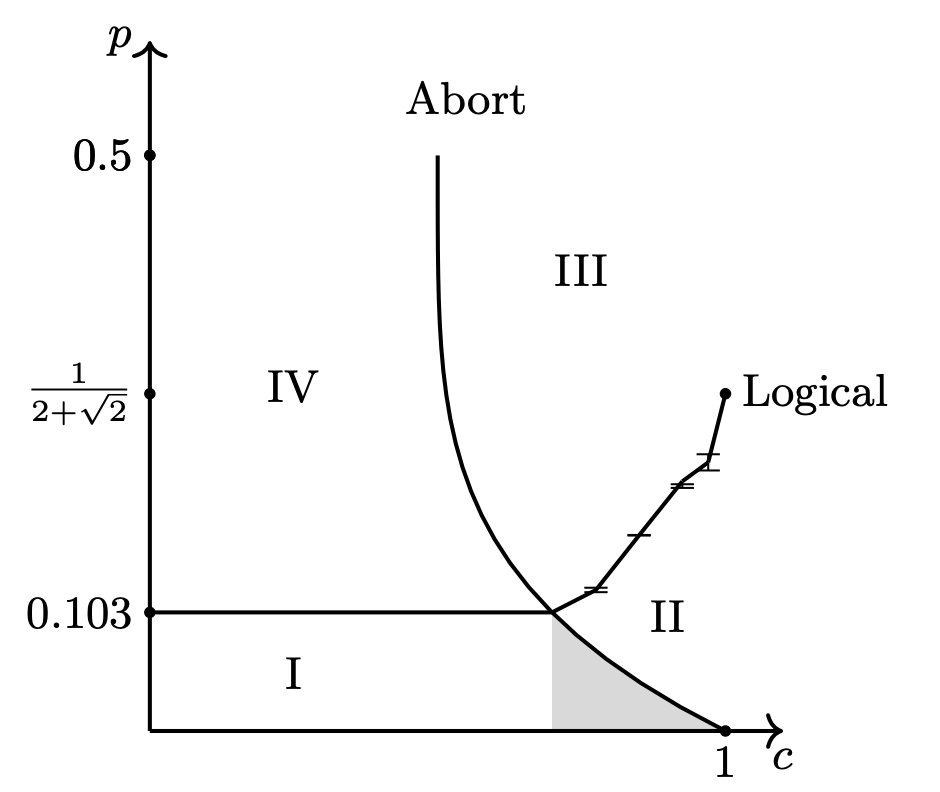
\includegraphics[width=.3\linewidth]{toric_code_phase_diagram.png}
\caption{Taken from \cite{english2024thresholdspostselectedquantumerror}. My rough understanding: Phase I is below both logical and abort thresholds (strong correlations). The shaded area is most interesting as it corresponds to increased logical threshold, while remaining below abort threshold.Phase I → Limited autonomous reachability (ordered phase with strong constraints).phase IV → Enhanced reachability (critical scaling with power-law bounds)
Phase III → Broader but bounded reachability (disordered phase)}
\end{figure}
\tom{TO DO: GIVE MORE DETAILS HERE}

Consider the statistical mechanical mapping where quantum codes correspond to disordered classical models with Hamiltonian:

\begin{equation}
    H_{stat}({\sigma_i}) = -\sum_{\langle i,j \rangle} J_{ij}(\vec{E}) \sigma_i \sigma_j - \sum_i h_i(\vec{E}) \sigma_i
\end{equation}


where disorder ${J_{ij}(\vec{E}), h_i(\vec{E})}$ depends on quantum error configuration $\vec{E}$.
I think there should be some sort of correspondence between phase boundaries in the statistical mechanical model and autonomous reachability.

For stabilizer codes with generators $\{S_\alpha\}$, autonomous initialization requires:
\begin{align}
\left\|\left|\psi_{\text{target}}\right\rangle - \exp\left(-i\sum_{k=1}^n \lambda_k H_k t\right)\left|\psi_{\text{init}}\right\rangle\right\| < \varepsilon
\end{align}
where $H_k$ are 2-body Hamiltonians and $|\psi_{\text{init}}\rangle$ is a product state.

More specifically different phases shown in fig. \ref{fig:toric_code_phase_diagram} should constrain reachability. Perhaps, we could even conjecture that $P_{reach}(\vec{\lambda})$ (as plotted in fig. \ref{}) follows:
\begin{equation}
    P_{reach}(\vec{\lambda}) \leq f\left(\frac{|\vec{\lambda}|}{|\vec{\lambda}_c|}\right) \exp\left(-\frac{|\vec{\lambda} - \vec{\lambda}_c|}{|\vec{\lambda}_c|}\right)
\end{equation}
where $\vec{\lambda}_c$ corresponds to the critical point in the mapped statistical model and $f$ is a universal scaling function.

\tom{THINK OF VERY SIMPLE EXAMPLES/SPECIFIC CODES TO SIMULATE AND TEST}

    \item \textbf{(Reachability $\rightarrow$ Decoding) Can we learn something about decoding using this mapping and our reachability conditions?}

    
\begin{figure}[!h]
\label{fig:threshold}
\centering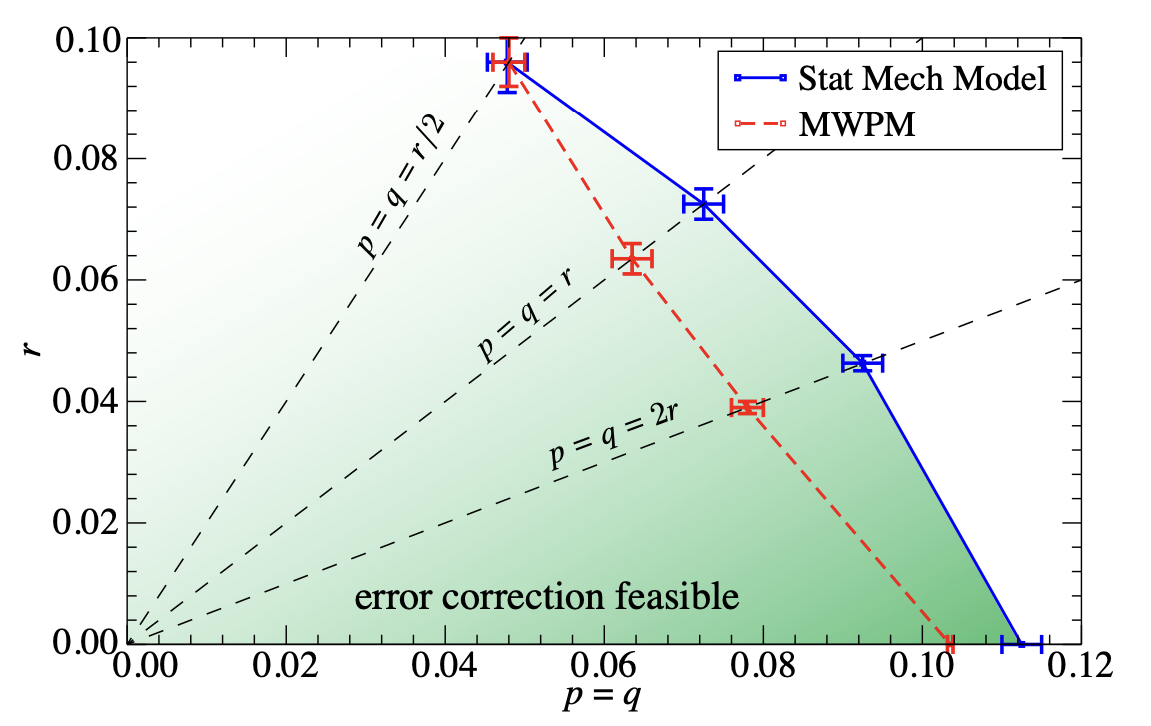
\includegraphics[width=.5\linewidth]{threshold.png}
\caption{Taken from \cite{Vodola_2022}. My rough understanding: }
\end{figure}


    In particular, could results of fig. \ref{fig:random_goe} (which say that some states are unreachable) be used to design a decoder that filters out unreachable states. That would be interesting as current decoders may frequently attempt corrections that are difficult to prepare.


Could we explain the gap between MWPM and stat mech model using our reachability criteria? The stat mech model assumes optimal maximum likelihood decoding which may require operations not implementable with autonomous $2$-body Hamiltonians. Filtering out unrealizable (as determined by theorem \ref{2}) corrections could maybe explain this gap or lead to a better decoder?

    \tom{TO DO: GIVE MORE DETAILS HERE}

    \textit{Decoder design}

    We could incorporate the reachability criteria into maximum likelihood decoder to filter out corrections that are difficult to prepare autonomusly. 

    \textit{Possible experiments}
    We could later compare our decoder with MWPM for repetition code, surface code and do some scaling analysis vs distance.

    \textit{Possible hurdles}

    Design of optimal decoders is usually difficult and stat mech decoder is known to be computationally expensive so our decoder could prove to expensive too :(

\item \textbf{(Decoding $\rightarrow$ Reachability) Can decoding teach us something about unreachability?}
    \tom{TO DO: GIVE MORE DETAILS HERE}

    Some potential parallels between decoding and autonomus reachability:
    \begin{itemize}
        \item Syndrome constraints in decoding map to moment constraints in autonomous reachability
        \item similar critical exponents nearconstraint satisfaction transitions
        \item NP-hard decoding instances could correpsond to probabiltiy of unreachability being higher
    \end{itemize}




\end{enumerate}



% \subsubsection{Graph states?}


% \subsubsection{Autonomous quantum error correction?}


\section{Interlude: Small-time evolution in $N$-qubit systems}
In the $N$-qubit system, with 2-body Hamiltonians described by \cref{eq:nqbham}, the initial evolution of $n$-sector lengths from any product state follows a universal pattern.
\begin{theorem}
\begin{equation}
A_n(\exp(-i\varepsilon H)\ket{\phi}) = \binom{N}{n} + \lambda\left(\binom{N-2}{n-1} - \binom{N-2}{n-2}\right)\varepsilon^2 + O(\varepsilon^4)
\label{eq:seclenev}
\end{equation}
where $\lambda$ depends on $H$ and $\ket{\phi}$, and
\begin{equation}
A_n := \sum_{1 \le i_1 < \ldots <i_n\le N} \sum_{(\alpha_i)} \langle \sigma^{(i_1)}_{\alpha_1} \cdot \ldots \cdot\sigma^{(i_n)}_{\alpha_n}\rangle^2,
\end{equation}
is called the $n$-sector length.
\end{theorem}
 This severely constrains short-time reachability -- although one could phrase it as "\emph{2-body Hamiltonians initially produce 2-body correlations}", I do not think this is the right interpretation. Note that the initial change is of order $\varepsilon^2$, and the correlation buildup is linear in time.
\begin{figure}[!h]
\centering
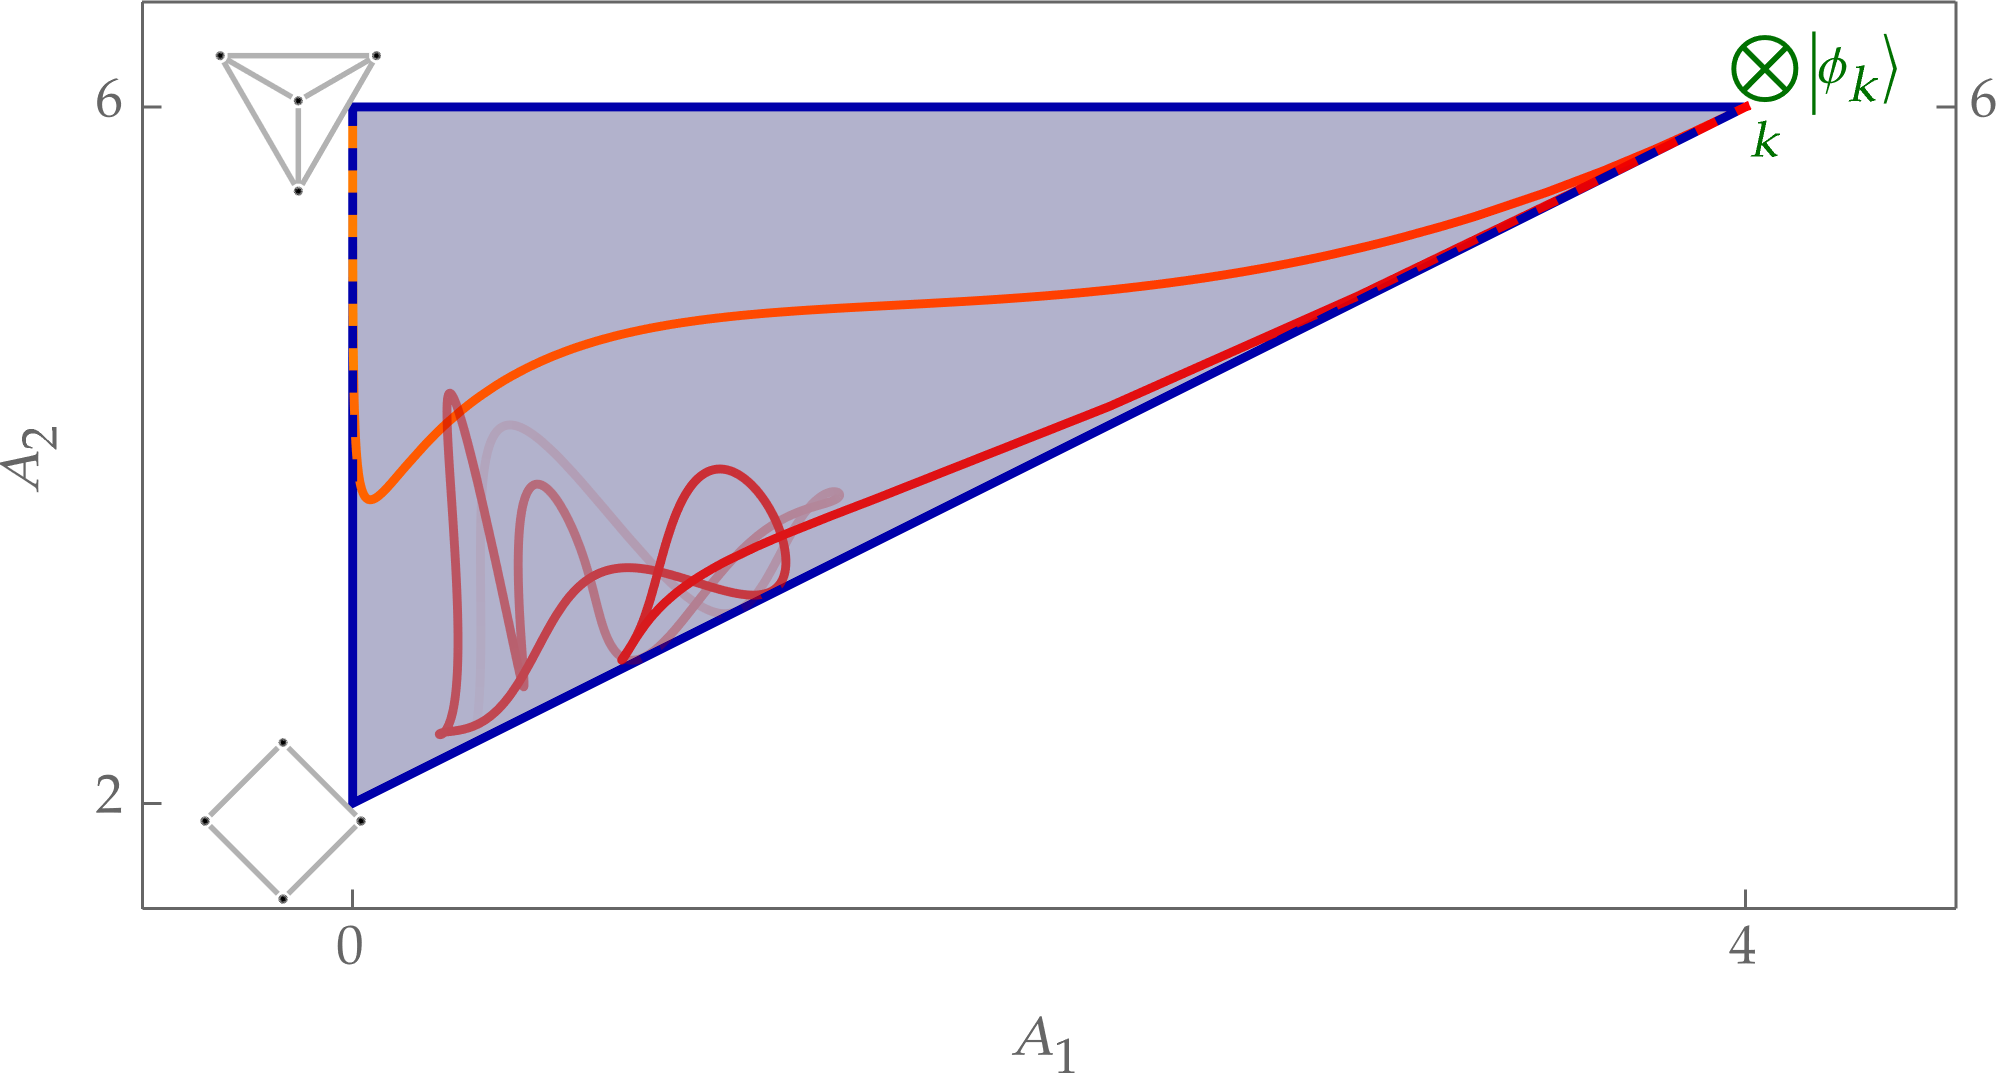
\includegraphics[width=.7\linewidth]{sectorlengths.png}
\caption{Evolution of sector lengths $A_1$ and $A_2$ for $4$-qubit system: the two trajectories: of a very specific initial state and Hamiltonian, leading to GHZ state (orange curve) and random initial product state and random 2-body Hamiltonian (red curve) are initially tangent, in accordance with \cref{eq:seclenev}. The set of all possible sector lengths for pure states is in this case a triangle, spanned by product states (right vertex, highlighted green text), GHZ state (top left vertex) and a square graph state (bottom left).}
\end{figure}
\section{Further questions}
The \cref{thm:twomom} is just a sufficient, but not necessary condition for unreachability. It is possible for the test to be unconclusive, in which case no statement about reachability can be made. It is due to the simplicity of the condition -- we use only the first two moments and a bit of linear algebra. But maybe it's possible to devise a stronger condition?
\begin{oquestion}
How to obtain computationally tractable unreachability conditions stronger than \cref{thm:twomom} derived from \cref{thm:allmom}?
\end{oquestion}

\cref{thm:allmom} is a stronger statement, but even this is just a sufficient condition for unreachability (and therefore necessary condition for reachability). Even when all moments match, and the Hamiltonian $H$ is nondegenerate, reachability requires that the orbit densely explores phase space. If $H\ket{n} = E_n\ket{n}$ and both states have decompositions differing only by phases:
\begin{equation}
\ket{\psi} = \sum_n \sqrt{p_n} e^{i\alpha_n}\ket{n}, \quad \ket{\phi} = \sum_n \sqrt{p_n} e^{i\beta_n}\ket{n}\end{equation}

Then $\ket{\psi}$ is reachable only if the phases $\{e^{-iE_n t}\}$ can approximate $\{e^{i(\alpha_n-\beta_n)}\}$ arbitrarily well.
\begin{oquestion} How can we decide if a given nondegenerate Hamiltonian $H$ can give rise to arbitrary phase structure through evolution? By Kronecker theorem, this is equivalent to the energies being rationally independent:
\begin{equation}
\sum_{n=1}^d \overbrace{m_n}^{\in\mathbb{Z}} E_n = 0 \implies (m_1, \ldots, m_d) = (0,\ldots,0).
\end{equation}
\end{oquestion}
The above question is related to Galois theory (since it is a statement about roots of the characteristic polynomial of $H$), which I unfortunately know nothing about.

The most important open question -- at least from the perspective of trying to write an interesting article! -- is about the physical relevance:
\begin{oquestion}
In what experimental contexts are autonomous Hamiltonians a natural restriction? Potential areas:
   \begin{itemize}
   \item natural time evolution in closed quantum systems,
   \item autonomous quantum computation,
   \item condensed matter physics (materials are rarely controlled from the outside).
   \end{itemize}
\end{oquestion}

\section{Ad hoc section to not forget about one interesting paper}

The paper \cite{QuantumAdvantage} starts from the same point, but goes into the direction of whether probability distribution resulting from by autonomous dynamics (local, $k$-qubit, with random interactions to make it mathematically concrete etc., starting from product states) are computationally tractable (spoiler alert: they are not). It's not what we are considering per se, but certainly interesting. I'd do the following:
\begin{itemize}
    \item cite \cite{QuantumAdvantage}, it's quite a fun paper,
    \item read in more detail, don't have much time now,
    \item see if there is anything relevant in the papers the author is citing, and whether a relevant paper cites \cite{QuantumAdvantage}.
\end{itemize}

\bibliographystyle{apsrev4-1fixed_with_article_titles_full_names_new}
\bibliography{reachability}


\end{document}